\section{Experiments}
\label{sec:experiments}

\subsection{Synthesized misannotation, misclassification and inexhaustive annotations}
\label{subsec:robustness}

%%%%%%%% TEXT
\noindent
\textit{Experiment setup}
\noindent
In order to investigate the influence of misannotation, misclassification and inexaustive annotation on feature transferability respectively, we set up experiments with a perfectly annotated dataset, PASCAL VOC2011\cite{everingham2015pascal}.
15 out of 20 categories were selected to form a \textit{pre-training dataset} and the other categories formed a \textit{fine-tuning dataset}.
The pre-training dataset was used to train Fully Convolutional Networks with AlexNet (FCN-AlexNet) models in the precense or absence of synthesized segmentation errors.
The fine-tuning dataset was used to fine-tune the weights of convolutional layers from the pre-trained FCN-AlexNet model.
The fine-tuned models were evaluated by the mean intersection over union ratio (mean IU) achieved with the test set of the fine-tuning dataset.
The performance of fine-tuning model comparing to the random-initialized model indicates transferability of the pre-trained weights,

\noindent
In order to avoid the influence of categories-splitting choice, the 20 categories of VOC2011 were divided equally into four folds and each fold was studied separately.
The exact partitions of categories are listed in Table \ref{tab:robustness}.

\noindent \textit{Experiment details}
\noindent
The training dataset was enriched with extra manual segmentations by Hariharan et al.\cite{hariharan2011semantic}
To keep the segmentation task simple, we used only single-object images for both pre-training dataset and fine-tuning dataset, resulting in 4000 training images of 20 categories in total.
In order to accelerate the training process, we subsampled the original images by four times.
Fully Convolutional Networks with AlexNet was used for experiments because its relatively short training time and the existence of an ImageNet model for AlexNet.
Only weights of convolutional filters in AlexNet were transfered from the pre-training phase to fine-tuning phase and the other layers were random initialized, with Xavier Initialization.
The ImageNet model and completely random weight initialization are the upper bound and lower bound respectively for various pre-trained weights summarized in Table \ref{tab:robustness}.
The default hyperparameters of FCN-AlexNet\cite{long2015fully} were kept unchanged.
Training run 240,000 iterations for pre-training phase, and 12,000 iterations for fine-tuning phase.


\noindent \textit{What Table \ref{tab:robustness} tell us.
How annotation errors are synthesized;
What are the results compared to noise-free counterparts;
How synthesization different from reality;
}

\noindent
Misannotation, misclassification and inexaustive annotation were synthesized and studied separately with stochastically corruption of the well-annotated pre-training dataset as decribed in Section \ref{subsec:formulation}.
The exact label transition probabilities are summarized in the following paragraphs.

\noindent \textit{Misannotation}
\noindent
As discussed in Section \ref{subsec:formulation}, misannotation errors in this experiment were synthesized by selecting one category as the target category and all the other 14 categories in the pretraining dataset became non-target.
In the presence of misannotation errors, instances from non-target categories were misannotated as if they were also from the target category with probability of $p(\tilde{y_{ij}}=1 \vert y_{ij}=0) = 1$ and $p(\tilde{y_{ij}}=1 \vert y_{ij}=0) = 0.5$.
The two choices of probability result in the two pre-trained models, ``AllMisannotated'' model and ``HalfMisannotated'' model, in Table \ref{tab:robustness} respectively.
The noise-free case for misannotation is the datasets with only the selected target category segmented and the other 14 categories unsegmented, denoted as \textit{SingleTarget} in Table \ref{tab:robustness}.
{TODO results}

\noindent \textit{Misclassification}
\noindent
Misclassification errors were synthesized from the well-annotated pre-training dataset as well, as described in Section \ref{subsec:formulation}.
Labels for target segments transited stochastically from one category to another with probability:
$$p(\tilde{y_{ij}}=l \vert y_{ij}=k) = \frac{1}{K}$$.
The resulted trained model was denoted as ``AllRandomLabels'' in Table \ref{tab:robustness}.
Similiarly, if half of the objects were assigned with random labels with uniform probability, the corresponding pre-trained model is called ``HalfRandomLabels'' model.
The noise-free counterpart of these two noisy models is the model trained with true labels, ``TrueLabels''.
$$p(\tilde{y_{ij}}=l \vert y_{ij}=k) = \delta(l-k)$$.
{TODO results}

\noindent \textit{Inexaustive}
\noindent
Train data with inexaustive annotations were synthesized by randomly converting labels of segmented objects to 0 with probability:
$p(\tilde{y_{ij}}=0 \vert y_{ij}=k) = 0.5$
{TODO results}

%%%%%%%% Table Learn Pixel Objectness for pre-training
\begin{table}[t]
\resizebox{\columnwidth}{!}{
\centering
\begin{tabular}{l|llll}
\makecell{Initial \\Representation}  & \makecell{mean IU \\(aeroplane,  \\bicycle, bird, \\boat, bottle)} & \makecell{mean IU \\(bus, car, \\cat, chair, \\cow)} & \makecell{mean IU \\ (dining table, \\dog, horse, \\motorbike, person)} & \makecell{mean IU \\(potted plant, \\sheep, sofa, \\train, TV)} \\
\hline
ImageNetModel    & \makecell{$0.42\pm0.01$} & \makecell{$0.51\pm0.01$} & \makecell{$0.49\pm0.01$} & \makecell{$0.47\pm0.01$} \\
RandomWeights    & \makecell{$0.29\pm0.01$} & \makecell{$0.29\pm0.03$} & \makecell{$0.27\pm0.01$} & \makecell{$0.30\pm0.02$} \\
\hline
SingleTarget     & \makecell{$0.26\pm0.01$} & \makecell{$0.37\pm0.03$} & \makecell{$0.27\pm0.01$} & \makecell{$0.33\pm0.04$} \\
AllMisannotated  & \makecell{$0.30\pm0.02$} & \makecell{$0.35\pm0.01$} & \makecell{$0.29\pm0.02$} & \makecell{$0.35\pm0.03$} \\
HalfMisannotated & \makecell{$0.26\pm0.00$} & \makecell{$0.33\pm0.00$} & \makecell{$0.30\pm0.00$} & \makecell{$0.33\pm0.00$} \\
\hline
TrueLabels       & \makecell{$0.29\pm0.01$} & \makecell{$0.36\pm0.01$} & \makecell{$0.29\pm0.01$} & \makecell{$0.37\pm0.01$} \\
AllRandomLabels  & \makecell{$0.29\pm0.01$} & \makecell{$0.33\pm0.03$} & \makecell{$0.26\pm0.01$} & \makecell{$0.28\pm0.01$} \\
HalfRandomLabels & \makecell{$0.27\pm0.01$} & \makecell{$0.33\pm0.02$} & \makecell{$0.25\pm0.01$} & \makecell{$0.29\pm0.01$} \\
\hline
InexaustiveLabels& \makecell{$0.26\pm0.01$} & \makecell{$0.30\pm0.3$} & \makecell{$0.28\pm0.03$} & \makecell{$0.32\pm0.02$} \\
\end{tabular}
}
\caption{Performances of fine-tuned FCN-AlexNet models with different representation initializations.
\textit{ImageNetModel} represents the pre-trained ImageNet model;
\textit{RandomWeights} indicates that the weights were randomly initialized;
All the other weights were first trained with the pre-training dataset in the presence or the absence of different types of label noises.
Each experiment was repeated three times, the mean and the standard deviation were computed over the last five snapshots for all repetitions.
% \textit{SingleCategory} was pre-trained on only one annotated category, either ``dog'' or ``cat'' depending on the fold, and the other categories were left unannotated;
% \textit{BinaryLabels} was pre-trained with binary labels that any objects of the fifteen categories were annotated as one single category, namely ``dog'' or ``cat'' depending on fold;
% \textit{TrueLabels} was pre-trained with all objects segmented and assigned to 15 categories correctly;
% \textit{AllRandomLabels} was pre-trained with all objects correctly segmented but assigned random labels;
% \textit{HalfRandomLabels} was pre-trained with all objects correctly segmented and half of them randomly assigned labels;
% \textit{IncompleteLabels} was trained with datasets that objects were annotated correctly with a probability of 0.5;
}
\label{tab:robustness}
\end{table}



\subsection{PU Learning for classification and for segmentation}
\label{subsec:pulearning}

%%%%%%%% FIGURE Varying positive annotating percetage
\begin{figure}[t]
\centering
   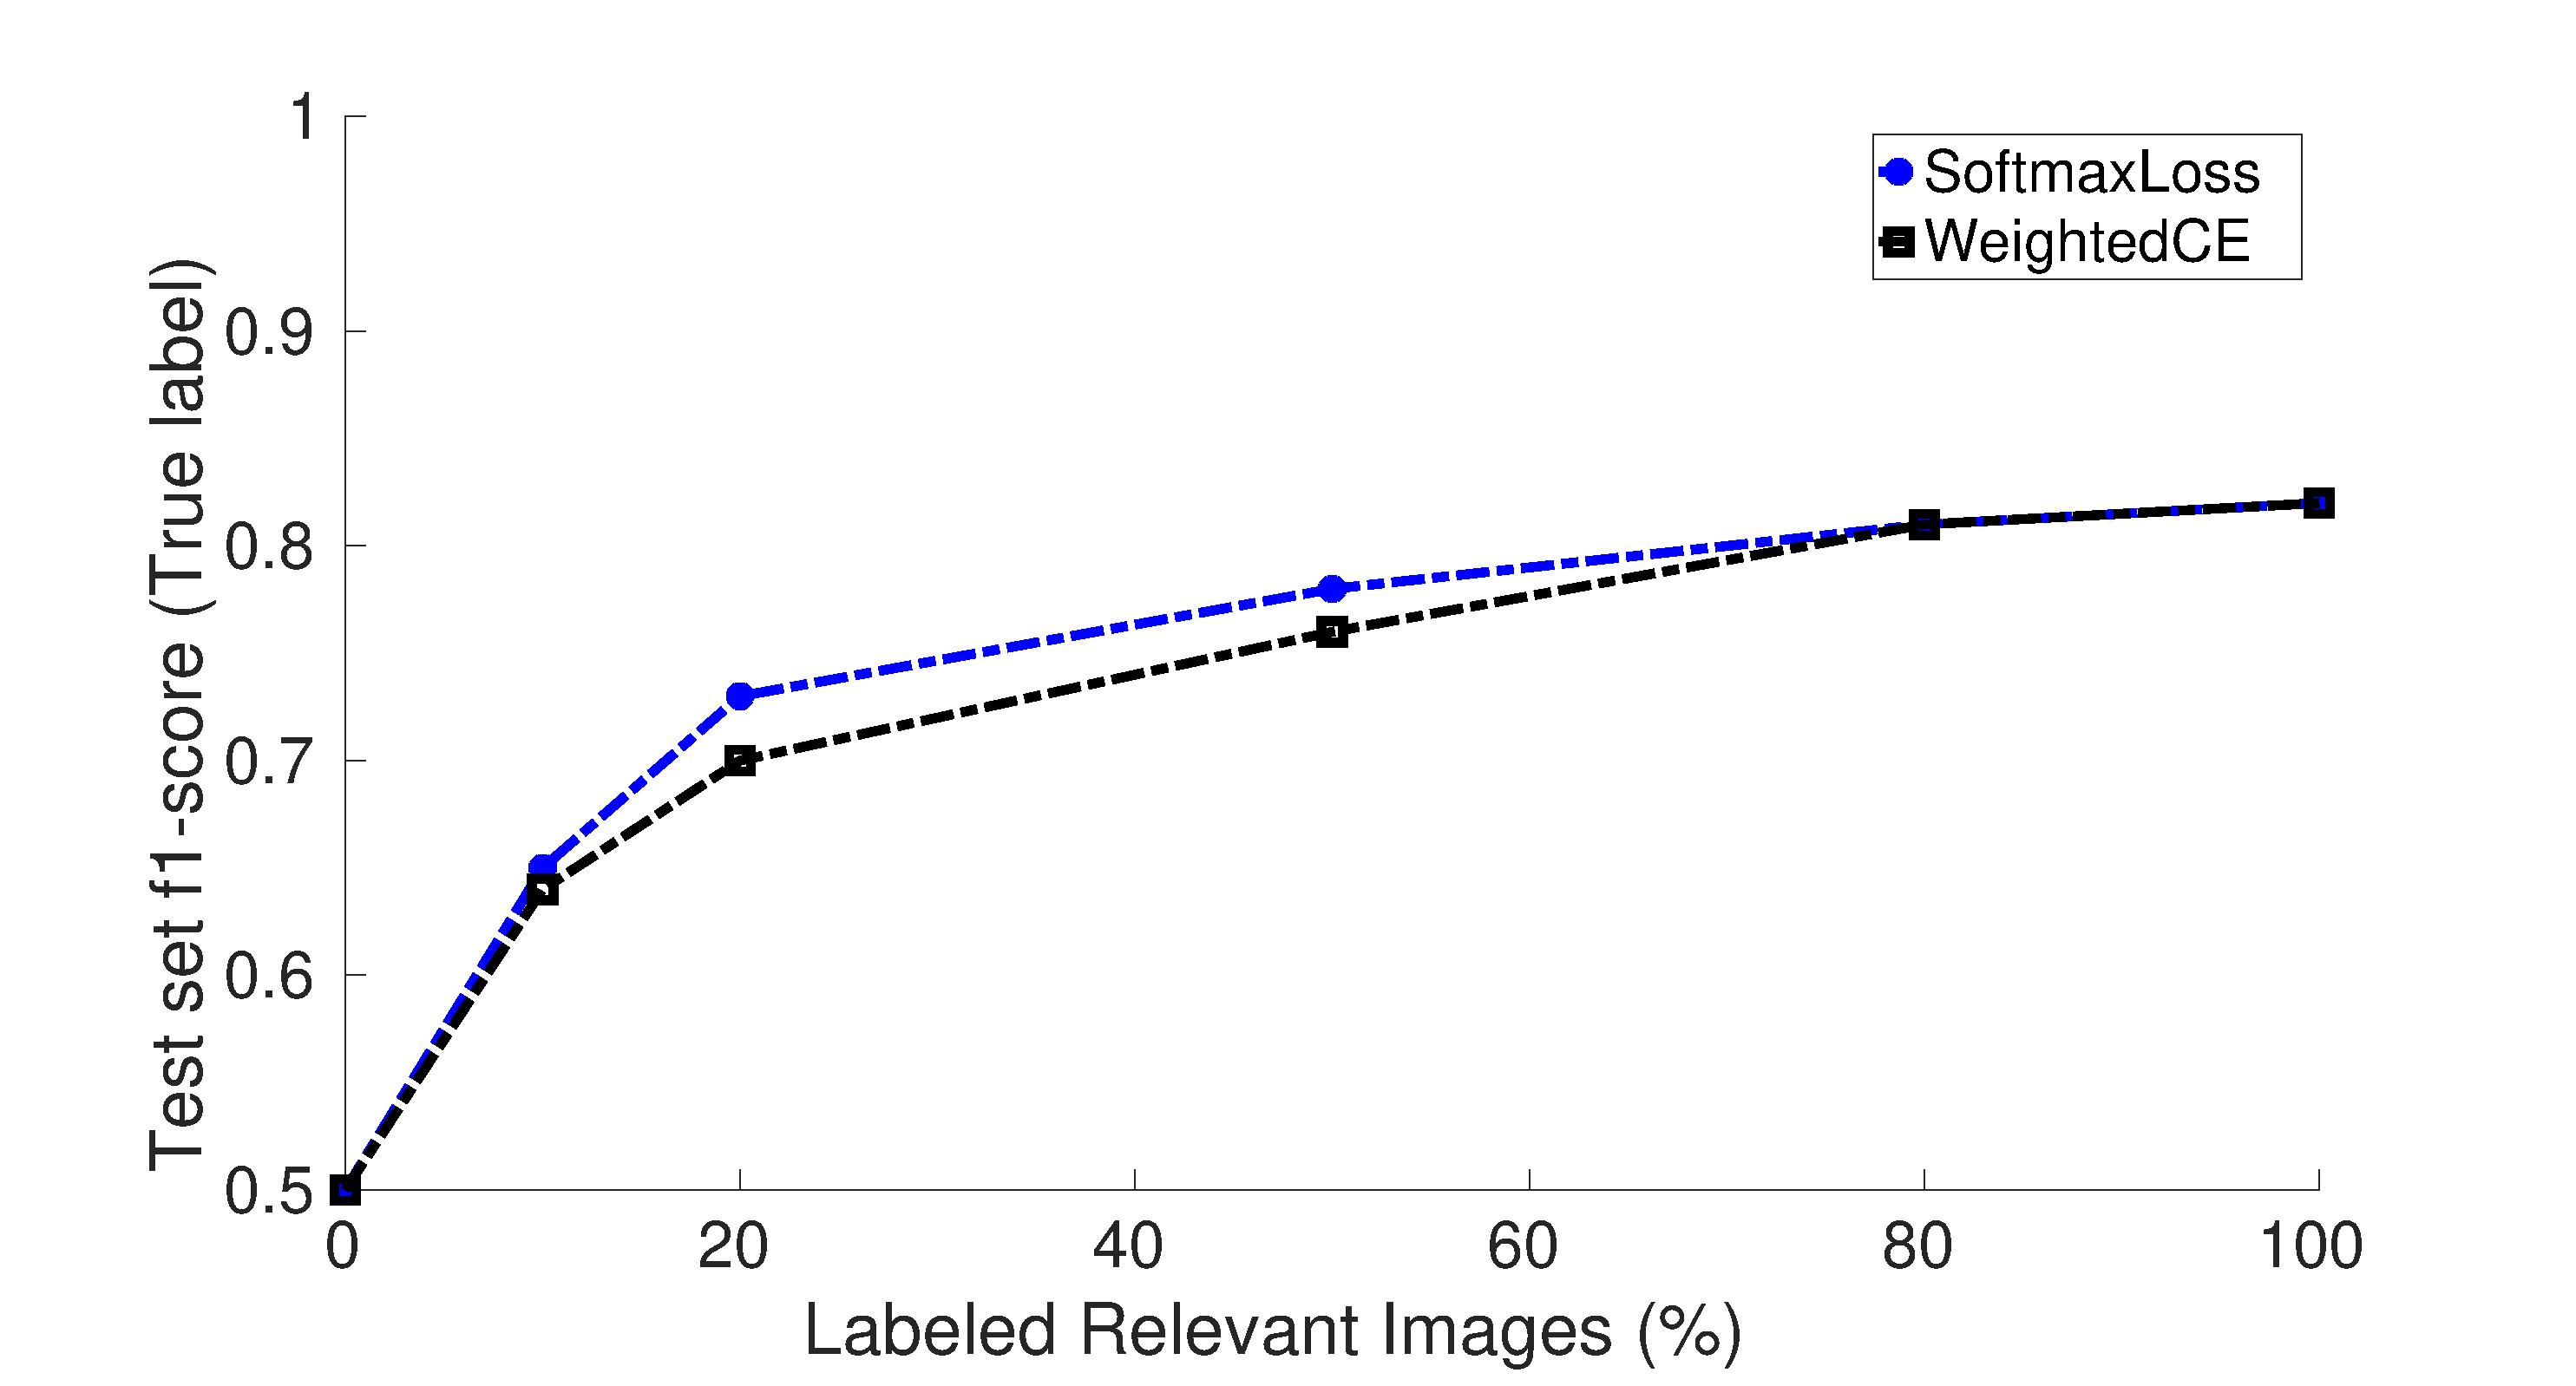
\includegraphics[width=\linewidth]{img/pu_vs_pn}
\caption{Varying percentage of annotated positives 10\%, 20\%, 50\%, 80\% and 100\% with images from CIFAR10 as the positives and images from CIFAR110 as the negatives.}
\label{fig:pct_annotating}
\end{figure}

%%%%%%%% TABLE CIFAR10
\begin{table}[t]
\resizebox{\columnwidth}{!}{
\centering
\begin{tabular}{ll|llll}
Annotation  & Loss & acc. & prec. & rec. & $F_1$ \\
\hline
Complete    & CrossEntropyU.   & 0.87 & 0.88 & 0.82 & 0.85 \\
50\%(P+N)   & CrossEntropyU.   & 0.83 & 0.84 & 0.78 & 0.80 \\
\hline
50\%P+U     & CrossEntropyU.   & 0.66 & 0.94 & 0.39 & 0.50 \\
50\%P+U     & WeightedU.       & 0.78 & 0.75 & 0.75 & 0.76 \\
50\%P+U     & ExponentialU.    & \textbf{0.81} & \textbf{0.85$\pm0.03$} & 0.72$\pm0.03$ & 0.77 \\
50\%P+U     & BootstrapHard    & 0.80 & 0.76 & \textbf{0.81} & \textbf{0.78} \\
\end{tabular}
}
\caption{Image classification with positive examples partially annotated. The complete dataset contains images from CIFAR10 as the \textbf{positive} (P) set and images from CIFAR110 as the \textbf{negative} (N) set. The unannotated positive examples from P set construct the \textbf{unlabeled} (U) set together with the N set. Experiments were repeated three times with random split of P set and U set, and standard deviations were around 0.01 if not explicitly mentioned.}
\end{table}

Training F-1 0.83 vs 0.81

%%%%%%%% TABLE
\begin{table}[t]
\resizebox{\columnwidth}{!}{
\centering
\begin{tabular}{ll|llll}
Annotation  & Loss & pixel acc. & mean acc. & mean IU & f.w. IU \\
\hline
Complete    & CrossEnt.U    &  &  & & \\
50\%P+U     & CrossEnt.U    & & & & \\
50\%P+U     & WeightedU        &  &  & & \\
50\%P+U     & ExponentialU     &  &  & & \\
50\%P+U     & BootstrapHard    &  &  & & \\
\end{tabular}
}
\caption{Image semantic segmentation with images contain single instance only from the PASCAL VOC2011 segmentation dataset. The complete \textbf{positive} (P) set denotes the foreground instances and the \textbf{negative} (N) set consists of the background. The unannotated instances from P set construct the \textbf{unlabeled} (U) set together with the N set.}
\end{table}
